\subsection{OPA Model}

The next level of complexity to add is to use electrical information about the grid as well as loading patterns to determine the power flows.  The loadings on particular elements have a large effect on the failure probability of the given element.  This type of model was done by three groups, Oak Ridge National Laboratory, Power System Engineering Research Center of Wisconsin University, and Alaska University.  This class of models will be called OPA models.  They look at the power transmission system and consider engineering and physical aspects, as well as economic, regulatory, and political responses to balckouts and increases in load.

In 2001, Dobson et. al \cite{dobson_2001} found that the opposition of the slow time scale force of growth in load and system capacity and fast time scale of cascading power failures and outages produced a dynamic equillibrium that can be seen in real world data.  Many real world complex systems can be seen to have this self-organized criticality property.  This criticality means that the blackout size distribution follows a power-law distribution, $f(x) = ax^k$ with an exponent of $-1.3 \pm 0.2$,  making large blackouts more likely.  In addition to criticality, it also appear to be in an equilibrium.  The distribution of blackout size has not changed in the past 30 years.  They argue that you can't study larges blackouts by looking at initial triggering events only, but you must look at the root cause, and deeper, long-term forces that drive the evolution of power system.

On a slow time scale, there are several things that happen to the electricity grid.  The first main force is the slow growth in load (around 0.7\% growth per year for first decade of 21st century \cite{eia_gov}).  This has the effect of reducing the available capacity margins on power lines and increasing the likelihood of failures as well as possibly further constraining economic dispatch.  While the slow time scale is progressing, random exogenous events, acts of nature, happen to outage individual components.  These possibly initiate large cascading failures and blackout portions of the system.  The engineering response to blackouts in operating policies, maintenance, equipment and controls have the effect of increasing margins on the slow time scale.  These forces push against each other and settle in an equillibrium.

The following parts go through the details of these forces mathematically.  These are drawn from several OPA papers \cite{dobson_2001}, \cite{carreras_2004},\cite{dobson_2007}.  

\subsubsection{Slow Time Scale}
The slow time scale is simplified by using days as the time step, represented by index $t$.  There are three main components to the slow dynamics.
\begin{enumerate}
\item The demand grows at the beginning of each day.  We have $d_{it} = \lambda d_{i \rho(t)}$ where $\rho(t)$ represents the preceding time period and $i$ is a vertex with a load demanding $d_{it}$ on day $t$ at peak load.  They used $\lambda = 1.00005$, which corresponds to a yearly growth rate of $1.8\%$ (the yearly average for 1980-2000).  To represent daily load fluctuations, all loads are multiplied by a random number $r$, such that $2-\gamma \le r \le \gamma$ with $1 \le \gamma \le 2$.
\item The response to blackouts is to upgrade the transmission system by increasing the maximum capacity of transmission lines.  If a line has overloaded in a blackout, the response is to increase its capacity so that $U_{et} = \mu U_{e \rho(t)}$ with $e$ being an edge with capacity $U_{et}$ on day t.  They varied $\mu$ between $1.01$ and  $1.1$.  This parameter simplifies all of the efforts that go into these responses including increasing the frequency of maintenance, changing operating policy, installing new equipment, and adjusting or adding alarms and controls.  These responses are modeled as happening before the next day, but in reality can take place over many different time scales.
\item The response to increased demand is to increase generator power so that all demand can be met.  First, they assume that increases in power is quantized and not continuous.  The quantity $\Delta G_t = \kappa ( D_t / n_g )$ represents the amount of power increase for a generator with $\kappa$ being a few percent, $n_g$ being the number of generators, and $D_t = \sum_{i \in \cV} d_{it}$ is the total demand for time period $t$.  In order to increase generation at a node $i$, we need $g_{it}^+ + \Delta G_t \le \sum_{e=(i,j) | e \in \cE} U_{et}$, that is, the increased power needs to be able to flow out of its neighborhood.  $g_{it}^+$ represents the maximum power generation at node $i$ on day $t$.  Power is continued to be added to eligible nodes, $g_{it}^+ \leftarrow g_{it}^ + + \Delta G_t$, until the generator capacity margin has risen above a prescribed level.  The generator capacity margin is defined by
\begin{equation}
\left(\frac{G-D}{D}\right)_t = \frac{\sum_i g_{it}^+ - D_0 e^{(\lambda-1)t} }{D_0 e^{(\lambda-1)t}}
\end{equation}
with $D_0 e^{(\lambda-1)t}$ being the average power demanded not including daily fluctuations.  The generator capacity margin is used to deal with daily fluctuations in demand.  The generator capacity margin of the U.S. has an estimated mean value between 15\% and 30\% \cite{carreras_2004}.
\end{enumerate}

These forces balance against system outages throughout time.  The outages were modeled as being possible to take place every day and begin with random events with a given probability.  The next section will go into detail about the cascading process that is possible after the random events take place.

\subsubsection{Fast Time Scale}

Individual blackouts triggered by random events (equipment failure, weather, vandalism, attack) can become widespread through a series of cascades. 
The initial goal of building this cascading failure model was to produce a list of lines that could plausibly be involved in cascading event.  It simplifies the process of cascading failures considerable but is still able to capture important effects of topology changes throughout the process.  Figure \ref{fig:cascade} gives a quick overview of the fast time scale simulation used to model cascading power failures.

\begin{figure}
\centering
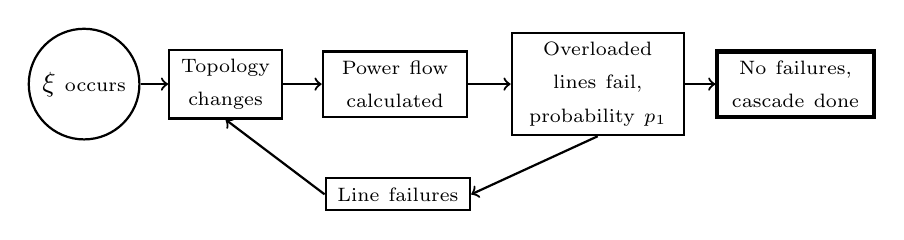
\begin{tikzpicture}
\draw [->,thick] (1,1) node[anchor=east, circle, draw]{$\xi$ \scriptsize occurs}
-- (1.35,1) node(TC)[anchor=west,text width=1.2cm,text centered,  rectangle, draw]{\scriptsize Topology changes};
\draw[->,thick] (TC)
--(3.3,1) node(PF)[anchor=west,text width=1.6cm,text centered, rectangle,draw]{\scriptsize Power flow calculated};
\draw[->,thick] (PF)
--(5.7,1) node(F)[anchor=west,text width=1.95cm, text centered, rectangle, draw]{\scriptsize Overloaded lines fail, probability $p_1$};
\draw[->,thick] (F)
--(8.3,1) node(DN)[anchor=west,text width=1.75cm, text centered,rectangle,draw,line width=1.5pt]{\scriptsize No failures, cascade done};
\draw[->,thick] (F.south)
--(5.2,-.4) node(LF)[anchor=east,text width=1.6cm, text centered, rectangle, draw]{\scriptsize Line failures };
\draw[->,thick] (LF.west)
-- (TC.south);

\end{tikzpicture} 
\caption{OPA simulation of a cascading power failure}
  \label{fig:cascade}
\end{figure}


The OPA model of the cascade process begins with an exogenous event, $\xi$, that effects the topology of the grid.  In their initial version, $\xi$ were the branches that randomly failed in an independent and identically distributed (I.I.D) manner, a Bernoulli trial with probability $p_0$.  Moments after the outage, the power flows are rerouted through the new topology based on the laws of physics.  In a longer time frame, it is possible for operators to take actions such as load shed and generator redispatch.  The resulting loading on the transmission lines is evaluated.  Their model then failed overloaded transmission lines with a Bernoulli trial with probability $p_1$ between  0.1 and 1.  After all overloaded lines are tried, a transition is made to the next stage.  Either there are no more outages, in which case the cascade is over, or more branch elements are outaged, the topology changes, and the operator is allowed to take recourse.  This process repeats until the system is stable and no outages occur.  Figure \ref{fig:cascade-example} shows a visual example of the cascading process.

For a given grid $\cG$ and initial demand $d_0$
\begin{description}
\item[ Initial $ \xi $ ]  For $e=1,...,n_e$, draw $\omega$ from $U[0,1]$ and if $\omega \le p_0$, line $e$ is outaged.
\item[ ] \hspace{35px} \vdots 
\item[ Stage $m$ ]  Calculate the power flows $f_{m}$, a column containing the branch flows for all edges in $\cE$, by using DC power flow equations with demand vector $d_m$. 

For $e=1,...,n_e$, if branch flow $f_{em} \ge U_{em}$, draw $\omega$ from $U[0,1]]$ and if $\omega \le p_1$, outage line $e$.
\end{description}

%\documentclass{standalone}
%\begin{document}

\def \sc     { .65 }
\def \lw     { 1.25pt }

\begin{figure}
\centering
\begin{subfigure}[b]{.46\linewidth}
\begin{tikzpicture}[line width=\lw,scale=\sc]

\node[circle,fill=blue!20] (one) at (3,0) {\small 1};
\node[circle,fill=red!20] (two) at (5,0) {\small 2};
\node[rectangle,fill=green!20] (three) at (7,1) {\small 3};
\node[rectangle,fill=green!20] (four) at (5,1.75) {\small 4};
\node[rectangle,fill=green!20] (five) at (3,1.75) {\small 5};
\node[circle,fill=red!20] (six) at (2,3) {\small 6};
\node[rectangle,fill=green!20] (seven) at (5,3) {\small 7};
\node[circle,fill=red!20] (eight) at (3.85,3.45) {\small 8};
\node[rectangle,fill=green!20] (nine) at (7,3) {\small 9};
\node[rectangle,fill=green!20] (ten) at (5.85,4.1) {\small 10};
\node[rectangle,fill=green!20] (eleven) at (3.75,5) {\small 11};
\node[rectangle,fill=green!20] (twelve) at (2.35,5) {\small 12};
\node[rectangle,fill=green!20] (thirteen) at (.81,4.2) {\small 13};
\node[rectangle,fill=green!20] (fourteen) at (4,6) {\small 14};


\draw (one) -- (two) ;
\draw (one) -- (five);
\draw (two) -- (three) ; 
\draw (two) -- (four) ; 
\draw (two) -- (five) ; 
\draw (three) -- (four) ; 
\draw[red] (four) -- (five) ; 
\draw (four) -- (seven);
\draw (four) -- (nine);
\draw (five) -- (six) ; 
\draw (six) -- (eleven) ; 
\draw (six) -- (twelve) ; 
\draw (six) -- (thirteen) ; 
\draw (seven) -- (eight) ; 
\draw (seven) -- (nine) ; 
\draw (nine) -- (ten) ; 
\draw (nine) .. controls +(up:1.2cm) .. (fourteen) ;
\draw[red] (ten) -- (eleven); 
%\draw[red] (eleven) -- (twelve); 
\draw[red] (twelve) -- (thirteen);
\draw (thirteen) .. controls +(up:1.2cm) .. (fourteen) ; 
\end{tikzpicture}
\caption{Initial Event: The three red lines are outaged and the power flow redistributes.}
\end{subfigure}
\begin{subfigure}[b]{.46\linewidth}
\begin{tikzpicture}[line width=\lw,scale=\sc]

\node[circle,fill=blue!20] (one) at (3,0) {\small 1};
\node[circle,fill=red!20] (two) at (5,0) {\small 2};
\node[rectangle,fill=green!20] (three) at (7,1) {\small 3};
\node[rectangle,fill=green!20] (four) at (5,1.75) {\small 4};
\node[rectangle,fill=green!20] (five) at (3,1.75) {\small 5};
\node[circle,fill=red!20] (six) at (2,3) {\small 6};
\node[rectangle,fill=green!20] (seven) at (5,3) {\small 7};
\node[circle,fill=red!20] (eight) at (3.85,3.45) {\small 8};
\node[rectangle,fill=green!20] (nine) at (7,3) {\small 9};
\node[rectangle,fill=green!20] (ten) at (5.85,4.1) {\small 10};
\node[rectangle,fill=green!20] (eleven) at (3.75,5) {\small 11};
\node[rectangle,fill=green!20] (twelve) at (2.35,5) {\small 12};
\node[rectangle,fill=green!20] (thirteen) at (.81,4.2) {\small 13};
\node[rectangle,fill=green!20] (fourteen) at (4,6) {\small 14};

\draw[red] (one) -- (two) ;
\draw (one) -- (five);
\draw (two) -- (three) ; 
\draw[red] (two) -- (four) ; 
\draw (two) -- (five) ; 
\draw[red] (three) -- (four) ; 
%\draw (four) -- (five) ; 
\draw (four) -- (seven);
\draw (four) -- (nine);
\draw (five) -- (six) ; 
\draw (six) -- (eleven) ; 
\draw (six) -- (twelve) ; 
\draw (six) -- (thirteen) ; 
\draw (seven) -- (eight) ; 
\draw (seven) -- (nine) ; 
\draw (nine) -- (ten) ; 
\draw (nine) .. controls +(up:1.2cm) .. (fourteen) ;
%\draw (ten) -- (eleven); 
%\draw (twelve) -- (thirteen);
\draw (thirteen) .. controls +(up:1.2cm) .. (fourteen) ; 
\end{tikzpicture}
\caption{Stage 1: Lines 1-2, 2-4, and 3-4 are overloaded. Lines 1-2 and 3-4 fail, but line 2-4 remains in operation at an overloaded state. }

\end{subfigure}
\begin{subfigure}[b]{.46\linewidth}

\begin{tikzpicture}[line width=\lw,scale=\sc]

\node[circle,fill=blue!20] (one) at (3,0) {\small 1};
\node[circle,fill=red!20] (two) at (5,0) {\small 2};
\node[rectangle,fill=green!20] (three) at (7,1) {\small 3};
\node[rectangle,fill=green!20] (four) at (5,1.75) {\small 4};
\node[rectangle,fill=green!20] (five) at (3,1.75) {\small 5};
\node[circle,fill=red!20] (six) at (2,3) {\small 6};
\node[rectangle,fill=green!20] (seven) at (5,3) {\small 7};
\node[circle,fill=red!20] (eight) at (3.85,3.45) {\small 8};
\node[rectangle,fill=green!20] (nine) at (7,3) {\small 9};
\node[rectangle,fill=green!20] (ten) at (5.85,4.1) {\small 10};
\node[rectangle,fill=green!20] (eleven) at (3.75,5) {\small 11};
\node[rectangle,fill=green!20] (twelve) at (2.35,5) {\small 12};
\node[rectangle,fill=green!20] (thirteen) at (.81,4.2) {\small 13};
\node[rectangle,fill=green!20] (fourteen) at (4,6) {\small 14};

%\draw[red] (one) -- (two) ;
\draw (one) -- (five);
\draw (two) -- (three) ; 
\draw[red] (two) -- (four) ; 
\draw[red] (two) -- (five) ; 
%\draw[red] (three) -- (four) ; 
%\draw (four) -- (five) ; 
\draw (four) -- (seven);
\draw (four) -- (nine);
\draw (five) -- (six) ; 
\draw (six) -- (eleven) ; 
\draw (six) -- (twelve) ; 
\draw[red] (six) -- (thirteen) ; 
\draw (seven) -- (eight) ; 
\draw[red] (seven) -- (nine) ; 
\draw (nine) -- (ten) ; 
\draw (nine) .. controls +(up:1.2cm) .. (fourteen) ;
%\draw (ten) -- (eleven); 
%\draw (twelve) -- (thirteen);
\draw (thirteen) .. controls +(up:1.2cm) .. (fourteen) ; 
\end{tikzpicture}
\caption{Stage 2: On the new topology, lines 2-5, 6-13, and 7-9 become overloaded.  The cascade progresses by outaging lines 2-4 and 7-9.}
\end{subfigure}
\begin{subfigure}[b]{.46\linewidth}
\begin{tikzpicture}[line width=\lw,scale=\sc]


\node[circle,fill=blue!20] (one) at (3,0) {\small 1};
\node[circle,fill=red!20] (two) at (5,0) {\small 2};
\node[rectangle,fill=green!20] (three) at (7,1) {\small 3};
\node[rectangle,fill=green!20] (four) at (5,1.75) {\small 4};
\node[rectangle,fill=green!20] (five) at (3,1.75) {\small 5};
\node[circle,fill=red!20] (six) at (2,3) {\small 6};
\node[rectangle,fill=green!20] (seven) at (5,3) {\small 7};
\node[circle,fill=red!20] (eight) at (3.85,3.45) {\small 8};
\node[rectangle,fill=green!20] (nine) at (7,3) {\small 9};
\node[rectangle,fill=green!20] (ten) at (5.85,4.1) {\small 10};
\node[rectangle,fill=green!20] (eleven) at (3.75,5) {\small 11};
\node[rectangle,fill=green!20] (twelve) at (2.35,5) {\small 12};
\node[rectangle,fill=green!20] (thirteen) at (.81,4.2) {\small 13};
\node[rectangle,fill=green!20] (fourteen) at (4,6) {\small 14};

%\draw[red] (one) -- (two) ;
\draw (one) -- (five);
\draw (two) -- (three) ; 
%\draw[red] (two) -- (four) ; 
\draw[red] (two) -- (five) ; 
%\draw[red] (three) -- (four) ; 
%\draw (four) -- (five) ; 
\draw[red] (four) -- (seven);
\draw[red] (four) -- (nine);
\draw (five) -- (six) ; 
\draw (six) -- (eleven) ; 
\draw (six) -- (twelve) ; 
\draw[red] (six) -- (thirteen) ; 
\draw (seven) -- (eight) ; 
%\draw[red] (seven) -- (nine) ; 
\draw (nine) -- (ten) ; 
\draw (nine) .. controls +(up:1.2cm) .. (fourteen) ;
%\draw (ten) -- (eleven); 
%\draw (twelve) -- (thirteen);
\draw[red] (thirteen) .. controls +(up:1.2cm) .. (fourteen) ; 
\end{tikzpicture}
\caption{Stage 3: This has the effect of routing all power destined for load 8 through the north passage. Lines 13-14, 4-7, and 4-9 are outaged along the path. }
\end{subfigure}

\begin{subfigure}[b]{.46\linewidth}
\begin{tikzpicture}[line width=\lw,scale=\sc]


\node[circle,fill=blue!20] (one) at (3,0) {\small 1};
\node[circle,fill=red!20] (two) at (5,0) {\small 2};
\node[rectangle,fill=green!20] (three) at (7,1) {\small 3};
\node[rectangle,fill=green!20] (four) at (5,1.75) {\small 4};
\node[rectangle,fill=green!20] (five) at (3,1.75) {\small 5};
\node[circle,fill=red!20] (six) at (2,3) {\small 6};
\node[rectangle,fill=green!20] (seven) at (5,3) {\small 7};
\node[circle,fill=red!20] (eight) at (3.85,3.45) {\small 8};
\node[rectangle,fill=green!20] (nine) at (7,3) {\small 9};
\node[rectangle,fill=green!20] (ten) at (5.85,4.1) {\small 10};
\node[rectangle,fill=green!20] (eleven) at (3.75,5) {\small 11};
\node[rectangle,fill=green!20] (twelve) at (2.35,5) {\small 12};
\node[rectangle,fill=green!20] (thirteen) at (.81,4.2) {\small 13};
\node[rectangle,fill=green!20] (fourteen) at (4,6) {\small 14};


%\draw[red] (one) -- (two) ;
\draw (one) -- (five);
\draw (two) -- (three) ; 
%\draw[red] (two) -- (four) ; 
\draw[red] (two) -- (five) ; 
%\draw[red] (three) -- (four) ; 
%\draw (four) -- (five) ; 
%\draw (four) -- (seven);
%\draw (four) -- (nine);
\draw (five) -- (six) ; 
\draw (six) -- (eleven) ; 
\draw (six) -- (twelve) ; 
\draw (six) -- (thirteen) ; 
\draw (seven) -- (eight) ; 
%\draw[red] (seven) -- (nine) ; 
\draw (nine) -- (ten) ; 
\draw (nine) .. controls +(up:1.2cm) .. (fourteen) ;
%\draw (ten) -- (eleven); 
%\draw (twelve) -- (thirteen);
%\draw (thirteen) .. controls +(up:1.2cm) .. (fourteen) ; 
\end{tikzpicture}
\caption{Stage 4:  Finally, line 2-5 that is still overloaded is outaged. }
\end{subfigure}
\begin{subfigure}[b]{.46\linewidth}
\begin{tikzpicture}[line width=\lw,scale=\sc]


\node[circle,fill=blue!20] (one) at (3,0) {\small 1};
\node[circle,fill=red!20] (two) at (5,0) {\small 2};
\node[rectangle,fill=green!20] (three) at (7,1) {\small 3};
\node[rectangle,fill=green!20] (four) at (5,1.75) {\small 4};
\node[rectangle,fill=green!20] (five) at (3,1.75) {\small 5};
\node[circle,fill=red!20] (six) at (2,3) {\small 6};
\node[rectangle,fill=green!20] (seven) at (5,3) {\small 7};
\node[circle,fill=red!20] (eight) at (3.85,3.45) {\small 8};
\node[rectangle,fill=green!20] (nine) at (7,3) {\small 9};
\node[rectangle,fill=green!20] (ten) at (5.85,4.1) {\small 10};
\node[rectangle,fill=green!20] (eleven) at (3.75,5) {\small 11};
\node[rectangle,fill=green!20] (twelve) at (2.35,5) {\small 12};
\node[rectangle,fill=green!20] (thirteen) at (.81,4.2) {\small 13};
\node[rectangle,fill=green!20] (fourteen) at (4,6) {\small 14};


%\draw[red] (one) -- (two) ;
\draw (one) -- (five);
\draw (two) -- (three) ; 
%\draw (two) -- (four) ; 
%\draw[red] (two) -- (five) ; 
%\draw[red] (three) -- (four) ; 
%\draw (four) -- (five) ; 
%\draw (four) -- (seven);
%\draw (four) -- (nine);
\draw (five) -- (six) ; 
\draw (six) -- (eleven) ; 
\draw (six) -- (twelve) ; 
\draw (six) -- (thirteen) ; 
\draw (seven) -- (eight) ; 
%\draw[red] (seven) -- (nine) ; 
\draw (nine) -- (ten) ; 
\draw (nine) .. controls +(up:1.2cm) .. (fourteen) ;
%\draw (ten) -- (eleven); 
%\draw (twelve) -- (thirteen);
%\draw (thirteen) .. controls +(up:1.2cm) .. (fourteen) ; 
\end{tikzpicture}
\caption{Stage 5:  The system stabilizes into islands with generator 1 serving load 6.  However, loads 2 and 8 are out of service.}
\end{subfigure}
\caption{ \label{fig:cascade-example} \small An example of a cascading power failure. Node 1 is a generator and nodes 2, 6, and 8 are loads.}
\end{figure}

%\end{document}


\subsubsection{Dynamic Equillibrium}

These opposing forces eventually find an equillibrium.  The equillibrium tends to be near critical points, which are points that have maximum power flow through the network for the nominal system capacity.  The system self-organizes towards these points which maximize efficiency of its assets.  When the system approaches these critical points, the power flow becomes limited due to two possible causes. 
\begin{itemize}
\item The power flows are limited due to tranmission line constraints.  This type of critical point has larger blackouts but happen less frequently.  In addition, the blackouts typically have  multiple lines tripping.
\item The power flows are limited due to generation capacity.  This results in frequent blackouts but of smaller size.
\end{itemize}
However, it is also possible to be in an operating regime which is close to both types of critical points simultaneously.  When this is the case, blackouts of all sizes occur.  While this operating regime may not be good from a reliability standpoint, it has the desirable characteristic of being able to deliver the maximum power for the system.   That is, when these two points are balanced, the system is capable of maximum throughput from its generators to its loads with minimal excess capacity.  This is important from an economic perspective and a critical reason the system self-organizes to these types of points.  This type of point tends to be the cheapest way to supply all the loads with power, while statisfying the minimum system reliability standards.

\subsubsection{Additional Complexities}

The OPA model can be extended to include additional complexities for many different reasons.  It is always a balance of how much resources you have to solve the problem and the amount of resolution you need in the solution.  The base OPA model is easy and fast to replicate, however by trying to gain increased resolution in the output, the model becomes increasingly complex and difficult to solve in a timely manner.

In related work, Chen et. al. \cite{chen_2005} find many similar conclusions to the OPA model by using an extension which included a hidden failure model.  A hidden failure is undectable in normal operations, but as the system becomes disturbed, a relay may incorrectly trip.  These protective relays are in operation to protect the line from overloads and disconnect it from the system.  This work introduces a loading dependent failure model that trips neighboring lines to outaged components.  This hidden failure is exposed the first time a disturbence nearby occurs and if it doesn't fail then, it is assumed to be properly operating and future disturbances will not undergo this hidden failure mechanism.  The probability of these happen in the real world are non-negligble according to NERC data \cite{nerc_dawg}.  

This work displays many similar results to the OPA papers.  First, the power law behavior near critical loading can be seen by varying the system loading levels.  They find that by increasing spinning reserves the risk of big blackouts is greatly reduced.  The blackout size distribution tends towards an exponential distrubition as reserve levels are increased.  By lowering the hidden failure rate, the system becomes more robust and larger blackouts become less likely.  Finally, they note that prompt control actions can reduce the risk of big disturbances.  While all of these results seem fairly straightforward, it points to the fact that the important aspects of the cascading process are being modeled and the effects are similar to what would happen in the real world.

Bienstock made several modifications \cite{bienstock_2011} to the original OPA model in order to remove some undesirable effects of the simulation, notably the erratic behavior of its output under small changes in the input.  To do this, he introduced the concept of memory to the system.  In order to see if a line is in or near an overloaded state, it uses a running time average of the current state and previous states.
\begin{equation}
\tilde{f}_{et} = \alpha f_{et} + (1-\alpha) \tilde{f}_{e\rho(t)}
\end{equation} 
Here, $f_{et}$ represents the power flow on edge $e$ at time $t$.  Then, $\tilde{f}_{et}$ is used in the overload and outage calculations.

In addition to including a memory, he also smoothed out the definition of an overloaded line by creating a step in between normal and overloaded states in which the failure probability was more than nominal but less than in the overloaded state.  Using $0 \le \epsilon \le 1$, for edge $e$, the following failure model smooths the effects of overloaded lines failing.
\begin{align}
\tilde{f}_{et} \ge (1+\epsilon) U_{et}			&	\hspace{10pt} \mbox{The line outages with certainty} 	\\
(1-\epsilon) U_{et} < \tilde{f}_{et} < (1+\epsilon) U_{et}	&	\hspace{10pt} \mbox{The line outages with probability }\frac{1}{2} 	\\
\tilde{f}_{et} \le (1-\epsilon) U_{et}			&	\hspace{10pt} \mbox{The line remains in operation} 
\end{align}

An AC power blackout model was developed at the University of Manchester (Manchester Model) by Nedic \cite{nedic_2006} and the original OPA authors.  This model is able to represent real world disturbances more accurately by using the full non-linear model that describes power flow.  This gives resolution into areas for generator instability, under-frequency load shedding, redispatch of active and reactive sources, and emergency load shedding.  The model has both automated control systems and operator recourse.  This model was used in OPA criticality works by Mei et. al. \cite{mei_2006}, including one with mechanisms using voltage stability margins \cite{mei_2008}.  However, the additional complexity comes at the cost of having to solve a nonlinear program and the loss of convergence gaureentees.  This is all done in order to represent something that is a companion too, but not the main driver of the cascading process (according to the Northeast outage working group, the main driver was angle instability not voltage instability).

Mei and others have worked to improve the accuracy of OPA by increasing the amount of details modeled \cite{mei_2009}.  In the fast dynamics, along with protective relays being modeled as hidden failures, they included a failure mechanism for the operational dispatch center that is responsible for generator redispatch.  In addition, they used a failure model where an underloaded line is failed with probability $p_1 \left( f_e/U_e \right)^N$, with $N=10$.  For the slow dynamics, they added a step that models a planning department by increasing the capacity of lines which have a loading rate $\left( f_{e}/ U_{e}  \right)$ greater than a set point.  

In 2013, Qi et. al. extended this model to include slow dynamics of vegetation growth and management.  Neglecting spatial variation and heating/cooling effects from   the environment, they model line temperature by a differential equation
\begin{equation}
\frac{dT(t)}{dt} = \alpha I^2 - \nu (T(t) - T_0)
\end{equation}
where $T(t)$ is the line temperature at $t$, $I$ current, $T_0$ initial temperature, and $\alpha$ and $\nu$ are calculated parameters.  This can be solved by assuming constant branch flow, $f$, to calculate the temperature over time
\begin{equation}
T(t) = e^{-\nu t}\left( T_0 - T_e(f) \right) + T_e(f)
\end{equation}
which can be used to find the final equilibrium temperature, $T_e(f)$ (a function of its constant power flow $f$ on the line), and time until a given temperature.  Using the calculated temperature, the horizontal span, and an elongation parameter, the line sag distance can be calculated.  When the minimum distance between lines and vegation passes a breakpoint based on transmission line characterestics such as operational voltage, the line will be outaged.  They model the vegetation with a daily growth rate model and include a managment simulation in which they identify future potential hazards and cut down trees over time.  The statistical analysis of there model aggreed well with historical data in China.

